\documentclass[11pt]{article}
\pagestyle{plain}
\usepackage[margin=1in]{geometry}
\usepackage{amsmath,amssymb,amsthm,booktabs}
\usepackage[T1]{fontenc}
\usepackage[utf8]{inputenc}
\usepackage{lmodern}
\usepackage{tikz}
\usepackage[hyphens]{url}
\usepackage[colorlinks=true,linkcolor=blue,citecolor=blue,urlcolor=blue]{hyperref}
\newtheorem{theorem}{Theorem}[section]
\newtheorem{lemma}[theorem]{Lemma}
\newtheorem{proposition}[theorem]{Proposition}
\newtheorem{corollary}[theorem]{Corollary}
\theoremstyle{definition}
\newtheorem{definition}[theorem]{Definition}
\newtheorem{example}[theorem]{Example}
\theoremstyle{remark}
\newtheorem{remark}[theorem]{Remark}
\numberwithin{equation}{section}
\newcommand{\Q}{\mathbb{Q}}
\newcommand{\N}{\mathbb{N}}
\newcommand{\ps}[1]{\Q[\![#1]\!]}
\newcommand{\m}{\mathfrak{m}}
\newcommand{\Oge}[1]{\mathcal{O}_{\geq #1}}
\newcommand{\Ole}[1]{\mathcal{O}_{\leq #1}}
\newcommand{\asc}{\textstyle\prod^{\rightarrow}}
\newcommand{\gl}{g_{<}}
\newcommand{\gr}{g_{>}}
\newcommand{\Sst}{S_{*}}
\newcommand{\bX}{\mathbf{X}}
\newcommand{\bY}{\mathbf{Y}}
\newcommand{\bZ}{\mathbf{Z}}
% Unicode characters appearing in the quoted Lean statement
\DeclareUnicodeCharacter{211A}{\ensuremath{\mathbb{Q}}}
\DeclareUnicodeCharacter{2265}{\ensuremath{\geq}}
\DeclareUnicodeCharacter{2264}{\ensuremath{\leq}}
\DeclareUnicodeCharacter{2203}{\ensuremath{\exists}}
\DeclareUnicodeCharacter{2200}{\ensuremath{\forall}}
\DeclareUnicodeCharacter{2227}{\ensuremath{\wedge}}
\DeclareUnicodeCharacter{2192}{\ensuremath{\to}}
\DeclareUnicodeCharacter{2211}{\ensuremath{\sum}}
\DeclareUnicodeCharacter{2208}{\ensuremath{\in}}
\setlength{\emergencystretch}{2em}
\raggedbottom
\title{A conjecture of Elgin, Reading and Stella on rank-two scattering coefficients}
\author{P. Graham\\ \small\url{https://orcid.org/0009-0007-8493-1505}}
\date{October 23, 2026}
\hypersetup{pdfauthor={P. Graham},pdftitle={A conjecture of Elgin, Reading and Stella on rank-two scattering coefficients}}
\begin{document}
\maketitle
\begingroup
\renewcommand{\thefootnote}{}
\footnotetext{The proofs, the Lean formalization and the text were produced by AI models (from OpenAI and Anthropic), working under the author's direction.}
\endgroup
\begin{abstract}
For positive integers $b$ and $c$, the rank-two cluster scattering
diagram $\mathfrak{D}(1+x^b,1+y^c)$ is the consistent scattering diagram
with initial walls $1+x^b$ and $1+y^c$; its wall functions have
coefficients $\tau^{b,c}(i,j)$. In 2024 Elgin, Reading and Stella stated
eighteen conjectures on these coefficients, supported by extensive
computation. Burcroff, Lee, Mou, Musiker and Reineke (2025) proved most of
them and recorded Conjecture~13 as unsolved and mysterious from both the
quiver-moduli and tight-grading points of view. We prove it, for the
coefficients as Burcroff et al.\ define them, which is the convention of
the table and code of Elgin, Reading and Stella: for every $j\geq1$,
$\tau^{1,5}(2j,j)=\frac1j\sum_{\ell}\binom{\ell}{j-\ell+1}\binom{j+\ell-1}{\ell}$.
After a change of lattice and a monomial substitution, the wall function
becomes the diagonal factor of the fifth power of an explicit automorphism
of $\Q[\![u,w]\!]$. A grading by the difference of the two degrees and the
Poisson bracket turn its factorization into a first-order differential
equation whose unique solution is algebraic. The proof is formalized in
Lean from the definitions.
\end{abstract}

\section{Introduction}\label{sec:intro}

Scattering diagrams were introduced by Kontsevich and Soibelman
\cite{KS06} and by Gross and Siebert \cite{GS11}, and became a central
tool for cluster algebras through the work of Gross, Hacking, Keel and
Kontsevich \cite{GHKK}. In rank two a scattering diagram is a collection of rays in
the plane, each carrying a power series called its wall function, subject
to a consistency condition (Section~\ref{sec:defs}). For positive integers
$b,c$ let $\mathfrak{D}(1+x^b,1+y^c)$ be the consistent diagram whose two
initial walls, on the coordinate axes, carry $1+x^b$ and $1+y^c$; it is
the rank-two cluster scattering diagram associated with the cluster
algebra $\mathcal{A}(b,c)$ \cite{GHKK,BLMMR}. Following
\cite[(2.2)]{BLMMR}, for coprime $d,e\geq1$ the coefficients
$\tau^{b,c}(kd,ke)$ are defined by expanding the wall function on the ray
of direction $(db,ec)$ as $1+\sum_{k\geq1}\tau^{b,c}(kd,ke)\,x^{kdb}y^{kec}$.

Elgin, Reading and Stella \cite{ERS} computed these coefficients
symbolically to high degree and stated eighteen conjectures about them
(first posted on arXiv on April~17, 2024, with Conjecture~13 already in
that version; published in 2026).
Their Conjecture~13 concerns $(b,c)=(1,5)$ and the wall of direction
$(2,5)$. Let
\[
  S(t)=1+\sum_{j\geq1}\tau^{1,5}(2j,j)\,t^j\in\ps{t},
\]
so that the wall function of $\mathfrak{D}(1+x,1+y^5)$ on the ray of
direction $(2,5)$ is $S(x^2y^5)$.

\begin{theorem}\label{thm:main}
For every $j\geq1$,
\begin{equation}\label{eq:ers}
  \tau^{1,5}(2j,j)=\frac1j\sum_{\ell=0}^{\infty}\binom{\ell}{j-\ell+1}\binom{j+\ell-1}{\ell},
\end{equation}
where only the terms with $\lceil (j+1)/2\rceil\leq\ell\leq j+1$ are
nonzero. Equivalently, $S=(1+\xi)/(1-\xi-\xi^2)$, where
$\xi\in t\ps{t}$ is the unique power series with $\xi=t+\xi^2+\xi^3$; and
$S$ is the unique power series with constant term $1$ satisfying
\begin{equation}\label{eq:cubic}
  t^2S^3-2tS^2+(1+t)S-(1+t)=0 .
\end{equation}
\end{theorem}

The first values are $\tau^{1,5}(2j,j)=2,5,17,64,259,1098,4815$ for
$j=1,\dots,7$. Theorem~\ref{thm:main} uses the convention for $\tau$ of
\cite{BLMMR}, which is the convention of the table and the code of
\cite{ERS}; Remark~\ref{rem:reading} explains this point.

The right side of \eqref{eq:ers} was known as a sequence before the
conjecture. Vladimir Kruchinin's OEIS entry A217596 (March 19, 2013), the
expansion of $x/\mathrm{reversion}(x-x^2-x^3)$, lists exactly this
binomial sum, so that the right side of \eqref{eq:ers} is
$-\mathrm{A217596}(j+1)$ \cite{OEIS}; in our notation its generating
function is $1-t\Sst$, with $\Sst$ the series of Theorem~\ref{thm:main}.
The same day Paul D. Hanna added functional equations for this
generating function $A$, the first being $A=1-t/A-t^2/A^2$; clearing
denominators gives the cubic $A^3=A^2-tA-t^2$, which Burcroff, Lee, Mou,
Musiker and Reineke used to note that the conjectured wall function is
algebraic \cite[\S9.3]{BLMMR}, and which is equivalent to
\eqref{eq:cubic} under $A=1-tS$. According to a comment of Muhammed
Sefa Saydam on the entry (January 27, 2025), $-\mathrm{A217596}(n)$ counts
the dissections of a convex $(n+2)$-gon into triangles and
quadrilaterals by noncrossing diagonals none of which passes through a
chosen vertex; so $\tau^{1,5}(2j,j)$ is this count for a $(j+3)$-gon
(for example $2$ for a square and $5$ for a pentagon). We do not use
this interpretation. What was open is that the scattering
coefficients equal these numbers; this is what Theorem~\ref{thm:main}
proves.

\subsection*{Prior work}
The conjectures, the data behind them and the code that produced the data
\cite{scatcoef} are due to Thomas Elgin, Nathan Reading and Salvatore
Stella \cite{ERS}. Amanda Burcroff, Kyungyong Lee, Lang Mou, Gregg
Musiker and Markus Reineke \cite{BLMMR} (first posted on arXiv on
November~18, 2025; published in 2026) proved Conjectures~1--3, 5--10 and
14--18 of \cite{ERS}, combining the change-of-lattice relation between
$\mathfrak{D}(1+x^b,1+y^c)$ and $\mathfrak{D}((1+x)^c,(1+y)^b)$ (from
\cite[Example~1.15]{GHKK}), Euler characteristics of quiver moduli through
the refined GW/Kronecker correspondence of Reineke and Weist \cite{RW},
and the tight gradings of Burcroff, Lee and Mou \cite{BLM}. They wrote
that Conjectures~4, 12 and~13 remain unsolved, and that the formula of
Conjecture~13 ``is mysterious from both the quiver moduli and tight
grading points of view'' \cite[\S1.3 of arXiv version~1]{BLMMR}. Ryota Akagi \cite{Akagi}
(first posted on arXiv on July~29, 2025)
proved Conjectures~1, 2, 3, 5, 6, 11 and~15 (the proof of~11 there is
due to Burcroff, Lee and Mou), with results related to 14 and 16--18, by
translating a description of rank-two cluster scattering diagrams through
dilogarithm elements into power series, building on his earlier explicit
forms of rank-two cluster scattering diagrams in low degrees
\cite{Akagi23} (first posted on arXiv on September~27, 2023). Amanda
Burcroff and Kyungyong Lee \cite{BL} study broken lines and compatible
pairs for rank-two quantum cluster algebras. The ordered-product
factorization on which everything rests is due to Kontsevich and
Soibelman \cite{KS06,KS08}; we use the formulation of Gross,
Pandharipande and Siebert \cite[\S1]{GPS}.

\subsection*{What is new}
The coefficients of a single wall are usually computed either by solving
the consistency equations degree by degree, which involves all walls at
once (this is how the data of \cite{ERS} were produced), or through
closed formulas for invariants attached to that wall, such as the Euler
characteristics and tight gradings used in \cite{BLMMR}. For the ray of
direction $(2,5)$ the first route gives only finitely many coefficients,
and, as recalled above, the authors of \cite{BLMMR} found no explanation
of the conjectured formula by the second. Here we
isolate this one wall. After the change of
lattice (Section~\ref{sec:lattice}) and the substitution $u=x$, $w=xy$
(Section~\ref{sec:T}), its fifth power becomes the diagonal factor $F$ in
the ordered factorization of $T^5$, where
$T=\theta_{(1,0),1+u}\circ\theta_{(0,1),1+w}$, a composition of two walls
(defined in \eqref{eq:wall}), is an explicit automorphism
of $\ps{u,w}$ that fixes $s=u+w$ and multiplies $u/w$ by $1+s$. The new
step, and the one that resisted, is to obtain a closed equation for $F$
without knowing the other walls. A grading by $h=(\text{degree in
}w)-(\text{degree in }u)$ separates the factors of slope below, at and
above the diagonal; writing $\gl$ for the product of the factors below the
diagonal, it shows that $P=\gl^{-1}(s)$ has only three
homogeneous components, $uF(uw)+\beta(uw)+w$ (Section~\ref{sec:filtration}).
Splitting $\log(1+P)$ by this grading determines $F$ in terms of one root
of a quadratic equation (Section~\ref{sec:split}), and the Poisson bracket
then turns the factorization into a first-order differential equation,
whose unique solution is algebraic (Sections~\ref{sec:string}
and~\ref{sec:solution}). We reuse the Kontsevich--Soibelman factorization,
the change of lattice (which we reprove in the form needed) and the
pentagon identity.

\subsection*{Organization}
Section~\ref{sec:defs} gives the definitions and the convention for $\tau$.
Section~\ref{sec:overview} outlines the proof. Section~\ref{sec:KS} proves
existence and uniqueness of ordered factorizations.
Sections~\ref{sec:lattice} and~\ref{sec:T} reduce the theorem to the
diagonal factor of $T^5$. Sections~\ref{sec:filtration}--\ref{sec:string}
derive a differential equation for that factor, and
Section~\ref{sec:solution} solves it and proves Theorem~\ref{thm:main}.
Section~\ref{sec:lean} describes the Lean formalization.

\section{Scattering diagrams and the coefficients \texorpdfstring{$\tau$}{tau}}\label{sec:defs}

This section fixes the definitions: walls, ordered products, consistency
and the coefficients $\tau^{b,c}$.

\subsection{Walls and ordered products}
Let $z_1,z_2$ be variables and $\mathcal{A}=\ps{z_1,z_2}$, with maximal
ideal $\m=(z_1,z_2)$ and the $\m$-adic topology. For $a\in\N^2$ write
$z^a=z_1^{a_1}z_2^{a_2}$ and $|a|=a_1+a_2$, and let
$\omega(a,r)=a_1r_2-a_2r_1$. A \emph{ray} is a primitive vector
$r\in\N^2\setminus\{0\}$, that is, one with $\gcd(r_1,r_2)=1$; rays are
ordered by their slope $r_2/r_1\in[0,\infty]$. Let
$\Lambda=1+t\ps{t}$ be the group of one-variable power series with
constant term $1$.

For a ray $r$ and $f\in\Lambda$, the \emph{wall} $\theta_{r,f}$ is the
continuous ring automorphism of $\mathcal{A}$ with
\begin{equation}\label{eq:wall}
  \theta_{r,f}(z_1)=z_1\,f(z^r)^{r_2},\qquad
  \theta_{r,f}(z_2)=z_2\,f(z^r)^{-r_1},\qquad\text{so}\qquad
  \theta_{r,f}(z^a)=z^a f(z^r)^{\omega(a,r)} .
\end{equation}
It is invertible, with $\theta_{r,f}^{-1}=\theta_{r,1/f}$, and walls on
the same ray compose by $\theta_{r,f}\theta_{r,g}=\theta_{r,fg}$. We
compose automorphisms as maps, $(\phi\psi)(\eta)=\phi(\psi(\eta))$. For
example, $\theta_{(1,0),1+t}$ fixes $z_1$ and sends $z_2$ to
$z_2/(1+z_1)$.

Since $f(z^r)-1\in\m^{|r|}$, a wall satisfies $\theta_{r,f}(\eta)-\eta\in\m^{|r|+1}$
for every $\eta\in\mathcal{A}$. Hence, modulo $\m^N$, only the finitely many
walls with $|r|<N$ act nontrivially. For a \emph{family}
$f=(f_r)$ of series $f_r\in\Lambda$, one for each ray, the
\emph{ascending product} $\asc_r\theta_{r,f_r}$ is the automorphism of
$\mathcal{A}$ that agrees, modulo $\m^N$ and for every $N$, with the
finite composition $\theta_{r^{(1)},f_{r^{(1)}}}\circ\theta_{r^{(2)},f_{r^{(2)}}}\circ\cdots$
over the rays with $|r|<N$ listed by increasing slope. Thus the ray of
smallest slope is leftmost and is applied last.

\subsection{Consistent diagrams}

\begin{definition}\label{def:consistent}
Let $P_1,P_2\in\Lambda$. A family $f=(f_r)$ is \emph{consistent for
$\mathfrak{D}(P_1,P_2)$} if
\begin{equation}\label{eq:consistent}
  \theta_{(0,1),P_2}\circ\theta_{(1,0),P_1}=\asc_r\theta_{r,f_r},
\end{equation}
where the product runs over all rays, including $(1,0)$ and $(0,1)$.
Equivalently, for every $N$ the two sides agree on $z_1$ and $z_2$ modulo
$\m^N$, the right side being the finite ascending product over $|r|<N$.
\end{definition}

By Proposition~\ref{prop:KS}, a consistent family exists and is unique.
Its entries on the axes are $f_{(1,0)}=P_1$ and $f_{(0,1)}=P_2$: on the
quotient $(z_2)/(z_2^2)$ every wall with $r_2\geq1$ acts as the identity
and $\theta_{(1,0),f}$ acts as multiplication by $f(z_1)^{-1}$, so
\eqref{eq:consistent} forces $f_{(1,0)}=P_1$, and symmetrically
$f_{(0,1)}=P_2$. Its function $f_r$ on a ray $r$ with $r_1,r_2>0$ is the
wall function on that ray of the diagram $\mathfrak{D}(P_1,P_2)$ of
\cite[\S2]{BLMMR} (Remark~\ref{rem:GPS}).

\begin{example}\label{ex:pentagon}
For $\mathfrak{D}(1+t,1+t)$ the consistent family has $1+t$ on the rays
$(1,0)$, $(1,1)$, $(0,1)$ and $1$ elsewhere: with
$\bX=\theta_{(1,0),1+t}$, $\bY=\theta_{(0,1),1+t}$ and
$\bZ=\theta_{(1,1),1+t}$, the identity $\bY\bX=\bX\bZ\bY$ holds, both
sides sending $z_1\mapsto z_1(1+z_2)$ and
$z_2\mapsto z_2/(1+z_1+z_1z_2)$. This is the pentagon identity.
\end{example}

\begin{definition}\label{def:tau}
Let $b,c\geq1$, let $f$ be the consistent family for
$\mathfrak{D}(1+t^b,1+t^c)$, and let $d,e\geq1$ be coprime. If $v$ is the
ray proportional to $(db,ec)$, then $f_v(z^v)$ is a series in
$x^{db}y^{ec}$, where $x=z_1$, $y=z_2$ \cite[\S2]{BLMMR}, and the
coefficients $\tau^{b,c}(kd,ke)$ are defined \cite[(2.2)]{BLMMR} by
\[
  f_v(z^v)=1+\sum_{k\geq1}\tau^{b,c}(kd,ke)\,x^{kdb}y^{kec}.
\]
\end{definition}

For $(b,c)=(1,5)$ and $(d,e)=(2,1)$ the vector $(db,ec)=(2,5)$ is
already a ray, so $\tau^{1,5}(2j,j)$ is the coefficient of $t^j$ in
$f_{(2,5)}(t)$, where $f$ is the consistent family for
$\mathfrak{D}(1+t,1+t^5)$. That is, $S=f_{(2,5)}$, the series of the
introduction. This is the only coefficient family used below.

\begin{remark}[Path-ordered products and orientation]\label{rem:GPS}
In \cite[\S1.3]{GPS}, crossing a wall supported on a line through $r$
acts by $z^a\mapsto z^a f^{\langle n_0,a\rangle}$, where $n_0\perp r$ is
primitive with $\langle n_0,\gamma'\rangle>0$ for the crossing path
$\gamma$, and a diagram is consistent when the path-ordered product
$\theta_{\gamma}=\theta_s\circ\cdots\circ\theta_1$ along every loop is the
identity. A counterclockwise loop starting just below the positive
$x$-axis crosses the positive $x$-axis, the rays $\mathbb{R}_{\geq0}r$ with
$r_1,r_2>0$ in order of increasing slope, and the positive $y$-axis, each
by $\theta_{r,f_r}^{-1}$ in the notation \eqref{eq:wall}, and then crosses
the negative $x$- and $y$-axes by $\theta_{(1,0),P_1}$ and
$\theta_{(0,1),P_2}$. So $\theta_\gamma=\mathrm{id}$ is the identity
$\theta_{(0,1),P_2}\theta_{(1,0),P_1}=\theta_{(1,0),P_1}\circ\big(\asc_{r_1,r_2>0}\theta_{r,f_r}\big)\circ\theta_{(0,1),P_2}$,
which is \eqref{eq:consistent}. Burcroff, Lee, Mou, Musiker and Reineke
draw the wall carrying $f_v$ on $\mathbb{R}_{\leq0}v$, in the sign
convention of \cite{GS11}, in which $z^a$ propagates in the direction
$-a$ (see \cite[\S1.2]{GPS}); the walls carry the same functions. As a
check on the orientation, Definition~\ref{def:consistent} with
$P_1=P_2=(1+t)^2$ gives $(1-t)^{-4}$ on the ray $(1,1)$ and $(1+t)^2$ on
$(n+1,n)$ and $(n,n+1)$, as found in \cite[\S1.3]{GPS}.
\end{remark}

\begin{remark}[Reading the definition in \cite{ERS}]\label{rem:reading}
The convention of Definition~\ref{def:tau} is that of the table of
$\tau^{3,2}(i,j)$, $0\leq i,j\leq7$, printed in \cite[\S2]{ERS}, all of whose entries it reproduces (we
compared them one by one), and of the code published with \cite{ERS}
(the method \texttt{wall\_hom} of \texttt{scatcoef.py} in \cite{scatcoef});
it is also the convention in which \cite{BLMMR} restate the conjectures.
A reader comparing with the definition in \cite[\S2]{ERS} should note that,
read literally, it attaches the exponents $b$ and $c$ to the two initial
walls the other way round, so that its coefficient $\tau^{b,c}(i,j)$
would be $\tau^{c,b}(i,j)$ in the convention used here. Under that
reading $\tau^{3,2}(3,1)$ would be $1$, whereas the table in \cite{ERS}
prints $0$, which is its value under Definition~\ref{def:tau}; and
Conjecture~13 would already fail at $j=1$, since $\tau^{5,1}(2,1)=0$. We
therefore read \cite{ERS} in the convention of its table and code.
\end{remark}

\section{Overview of the proof}\label{sec:overview}

This section outlines the argument; the details follow in the same order
in Sections~\ref{sec:KS}--\ref{sec:solution}.

\emph{Step 1: change of lattice (Section~\ref{sec:lattice}).} The ring
homomorphism $X\mapsto x$, $Y\mapsto y^5$ carries each wall of
$\mathfrak{D}_5:=\mathfrak{D}((1+t)^5,1+t)$, on $\ps{X,Y}$, to a wall of
$\mathfrak{D}(1+t,1+t^5)$. Comparing the two consistent families gives
$S^5=F$, where $F$ is the function of $\mathfrak{D}_5$ on the ray $(2,1)$.
This is a case of the change of lattice of \cite[Proposition~2.2]{BLMMR}.

\emph{Step 2: a single automorphism (Section~\ref{sec:T}).} On
$\ps{u,w}$ let $T=\theta_{(1,0),1+u}\circ\theta_{(0,1),1+w}$. The
substitution $u=X$, $w=XY$ carries walls to walls, $T$ to $\bX\bZ$, and
the ray $(1,1)$ to $(2,1)$. With the pentagon identity this shows that $F$
is the function on the diagonal ray $(1,1)$ in the ascending
factorization of $T^5$. Explicitly
\[
  T(u)=\frac{u(1+u+w)}{1+u},\qquad T(w)=\frac{w}{1+u},
\]
so $T$ fixes $s=u+w$ and $T(u)/T(w)=(1+s)\,u/w$.

\emph{Step 3: three components (Section~\ref{sec:filtration}).} Group the
factorization as $T^5=\gl\circ\theta_F\circ\gr$, the factors of slope
below~$1$, the diagonal wall $\theta_F=\theta_{(1,1),F}$, and the factors
of slope above~$1$. Give $u^pw^q$ the degree $h=q-p$. Walls of slope above
$1$ only add terms of positive $h$, and walls of slope below $1$ only
terms of negative $h$; the diagonal wall preserves $h$. Because $T^5$
fixes $s$, the series $P=\gl^{-1}(s)=\theta_F\gr(s)$ can be computed from
either side, and the two computations force
\[
  P=uF(t)+\beta(t)+w,\qquad t=uw,\quad \beta\in t\ps{t}.
\]
Nothing else about the infinitely many other walls is used.

\emph{Step 4: splitting the logarithm (Section~\ref{sec:split}).} The
ratio $\mu_\phi=(\phi(u)/u)/(\phi(w)/w)$ satisfies the cocycle rule
$\mu_{\phi\psi}=\phi(\mu_\psi)\,\mu_\phi$. Applied to $\gl^{-1}T^5=\theta_F\gr$ it gives
$(1+P)^5\,\mu_{\gl^{-1}}=F^2\,\theta_F(\mu_{\gr})$. Writing
$1+P=(1+u\delta)\,\rho\,(1+w/\rho)$ with $\rho,\delta\in\ps{t}$ and
comparing the parts of the logarithm with $h<0$, $h=0$ and $h>0$ yields
$F^2=\rho^5$ and $\mu_{\gl^{-1}}=(1+u\delta)^{-5}$.

\emph{Step 5: the string equation (Section~\ref{sec:string}).} The Euler
derivation $E=u\partial_u+w\partial_w$ satisfies $E(s)=s$; conjugating it by the
Poisson automorphism $\gl^{-1}$ shifts it by the Hamiltonian derivation of
$\log\mu_{\gl^{-1}}$. This gives $(1+u\delta)(E(P)-P)=5\{u\delta,P\}$,
and with $P=(\rho+w)(1+u\delta)-1$ the equation collapses to a single
first-order differential equation for $(\rho,\delta)$, with $\delta^2=\rho^3$,
which has exactly one solution.

\emph{Step 6: the solution (Section~\ref{sec:solution}).} The pair
$(\Sst^2,\Sst^3)$ with $\Sst=(1+\xi)/(1-\xi-\xi^2)$ solves the equation, so
$F=\Sst^5$ and $S=\Sst$; Lagrange inversion gives \eqref{eq:ers}.

The obvious approach, computing the factorization and recognizing the
coefficients, does not lead to a proof: in each degree the consistency
equations couple the wall of interest to all walls of smaller degree,
and many of them are nontrivial already in low degree
(Figure~\ref{fig:rays}). Steps~3--5 avoid them: the only information
about the other walls that enters is the sign of $h$ on each side of the
diagonal.

\section{Ordered factorization}\label{sec:KS}

This section proves the existence and uniqueness of ascending
factorizations (Proposition~\ref{prop:KS}), which make
Definition~\ref{def:consistent} meaningful and are used in every later
step.

\subsection{The Poisson bracket}
On $\mathcal{A}=\ps{z_1,z_2}$ let
\[
  \{f,g\}=(z_1\partial_{z_1}f)(z_2\partial_{z_2}g)-(z_2\partial_{z_2}f)(z_1\partial_{z_1}g),
  \qquad\text{so}\qquad \{z^a,z^b\}=\omega(a,b)\,z^{a+b}.
\]
It is a continuous biderivation, and $\{\log\eta,g\}=\{\eta,g\}/\eta$ for
$\eta\in1+\m$. An automorphism $\phi$ of
$\mathcal{A}$ is \emph{unipotent} if $\phi(z_i)\in z_i(1+\m)$ for
$i=1,2$, and \emph{Poisson} if $\phi\{f,g\}=\{\phi f,\phi g\}$ for all
$f,g$.

\begin{lemma}\label{lem:walls}
\begin{enumerate}
\item A unipotent automorphism $\phi$ is Poisson if and only if
$\{\phi(z_1),\phi(z_2)\}=\phi(z_1)\phi(z_2)$.
\item Every wall is a unipotent Poisson automorphism, and so is every
ascending product of walls.
\end{enumerate}
\end{lemma}

\begin{proof}
(1) By the chain rule, both $\phi\{f,g\}$ and $\{\phi f,\phi g\}$ equal
$\sum_{i,j}\phi(\partial_if)\phi(\partial_jg)$ times $\phi\{z_i,z_j\}$,
respectively $\{\phi z_i,\phi z_j\}$, and $\{z_1,z_2\}=z_1z_2$. (2) For
$g=f(z^r)$ one has $z_i\partial_{z_i}g=r_i\,q\,g$ with
$q=z^rf'(z^r)/f(z^r)$, and a direct computation gives
$\{z_1g^{r_2},z_2g^{-r_1}\}=z_1g^{r_2}\,z_2g^{-r_1}\big((1+r_1r_2q)(1-r_1r_2q)+r_1^2r_2^2q^2\big)=\theta_{r,f}(z_1)\,\theta_{r,f}(z_2)$,
so (1) applies. Products of unipotent Poisson automorphisms, and their
$\m$-adic limits, are again unipotent and Poisson.
\end{proof}

\begin{proposition}[Kontsevich--Soibelman]\label{prop:KS}
Let $\phi$ be a unipotent Poisson automorphism of $\mathcal{A}$. There is
exactly one family $f=(f_r)$ with $\phi=\asc_r\theta_{r,f_r}$. Moreover,
any automorphism of $\mathcal{A}$ has at most one such factorization.
\end{proposition}

\begin{proof}
We give the degree-by-degree argument of \cite{KS06} and
\cite[\S1.3]{GPS}. Say that two families agree below degree $d$ if
$[t^j]f_r=[t^j]f'_r$ whenever $j|r|<d$; then the corresponding ascending
products agree on $z_1,z_2$ modulo $\m^{d+1}$. If they agree below degree
$d$, then, since every wall is the identity to first order, the
coefficients of degree $d$ enter additively at the lowest order:
\begin{gather*}
  \asc\theta_{r,f_r}(z_1)-\asc\theta_{r,f'_r}(z_1)\equiv z_1\textstyle\sum r_2\,(c_{r,j}-c'_{r,j})\,z^{jr},\\
  \asc\theta_{r,f_r}(z_2)-\asc\theta_{r,f'_r}(z_2)\equiv -z_2\textstyle\sum r_1\,(c_{r,j}-c'_{r,j})\,z^{jr}
\end{gather*}
modulo $\m^{d+2}$, where the sums run over the pairs $(r,j)$ with
$j|r|=d$ and $c_{r,j}=[t^j]f_r$. Distinct pairs give distinct monomials
$z^{jr}$, and $(r_1,r_2)\neq0$, so this difference vanishes only if the
families agree below degree $d+1$. This proves uniqueness.

For existence, suppose that $\Pi=\asc\theta_{r,f_r}$ agrees with $\phi$
on $z_1,z_2$ modulo $\m^{d+1}$, with $d\geq1$, and write
$\phi(z_1)-\Pi(z_1)\equiv z_1\alpha$, $\phi(z_2)-\Pi(z_2)\equiv z_2\alpha'$
modulo $\m^{d+2}$, with $\alpha,\alpha'$ homogeneous of degree $d$. Both
$\phi$ and $\Pi$ satisfy Lemma~\ref{lem:walls}(1); subtracting the two
identities and keeping the terms of degree $d+2$ gives
$z_1z_2(z_1\partial_{z_1}\alpha+z_2\partial_{z_2}\alpha')=0$. So for
each monomial $z^k$ of degree $d$, the coefficients satisfy
$k_1\alpha_k+k_2\alpha'_k=0$, that is,
$(\alpha_k,\alpha'_k)=c_k\,(r_2,-r_1)$ with $r=k/\gcd(k_1,k_2)$. Adding
$c_k\,t^{\gcd(k_1,k_2)}$ to $f_r$ for each such $k$ changes the images of
$z_1,z_2$ only in degrees $\geq d+1$, and removes the discrepancy in
degree $d+1$. The resulting families converge coefficientwise, and their
limit factors $\phi$.
\end{proof}

By Lemma~\ref{lem:walls}, the left side of \eqref{eq:consistent} is
unipotent and Poisson, so every $\mathfrak{D}(P_1,P_2)$ has exactly one
consistent family.

\section{The change of lattice}\label{sec:lattice}

This section relates the ray $(2,5)$ of $\mathfrak{D}(1+t,1+t^5)$ to the
ray $(2,1)$ of $\mathfrak{D}_5=\mathfrak{D}((1+t)^5,1+t)$. The general
statement is the change of lattice of \cite[Proposition~2.2]{BLMMR},
going back to \cite[Example~1.15 and Appendix~C]{GHKK}; we prove the case
needed by a forward substitution.

Let $\mathfrak{D}_5$ live on $\ps{X,Y}$ and $\mathfrak{D}(1+t,1+t^5)$ on
$\ps{x,y}$, and let $\kappa\colon\ps{X,Y}\to\ps{x,y}$ be the injective
continuous ring homomorphism with $\kappa(X)=x$ and $\kappa(Y)=y^5$. For a
ray $(d,e)$ put
\[
  v(d,e)=\begin{cases}(d,5e)&\text{if }5\nmid d,\\ (d/5,e)&\text{if }5\mid d,\end{cases}
  \qquad
  G^{\kappa}_{(d,e)}(t)=\begin{cases}G(t)^{1/5}&\text{if }5\nmid d,\\ G(t^5)&\text{if }5\mid d,\end{cases}
\]
for $G\in\Lambda$, where $G^{1/5}$ is the unique fifth root in $\Lambda$.
The map $(d,e)\mapsto v(d,e)$ is a bijection of rays that multiplies
slopes by $5$, so it preserves their order.

\begin{lemma}\label{lem:kappa}
For every ray $(d,e)$ and $G\in\Lambda$,
$\kappa\circ\theta_{(d,e),G}=\theta_{v(d,e),G^{\kappa}_{(d,e)}}\circ\kappa$.
\end{lemma}

\begin{proof}
Both sides are continuous ring homomorphisms, so it suffices to compare
them on $X$ and $Y$. If $5\nmid d$, then $v=(d,5e)$,
$z^{v}=\kappa(X^dY^e)$ and $h=G^{1/5}$ give
$\theta_{v,h}(x)=x\,h(z^v)^{5e}=\kappa\big(X\,G(X^dY^e)^e\big)$ and
$\theta_{v,h}(y^5)=y^5h(z^v)^{-5d}=\kappa\big(Y\,G(X^dY^e)^{-d}\big)$. If
$5\mid d$, then $v=(d/5,e)$, $(z^v)^5=\kappa(X^dY^e)$ and $h(t)=G(t^5)$
give the same two values.
\end{proof}

\begin{proposition}\label{prop:lattice}
Let $G$ be the consistent family for $\mathfrak{D}_5$ and $f$ the
consistent family for $\mathfrak{D}(1+t,1+t^5)$. Then
$f_{(2,5)}^5=G_{(2,1)}$.
\end{proposition}

\begin{proof}
Define a family $f'$ on $\ps{x,y}$ by
$f'_{v(d,e)}=(G_{(d,e)})^{\kappa}_{(d,e)}$. By Lemma~\ref{lem:kappa},
applied to each wall, and continuity of $\kappa$,
$\kappa\circ\asc\theta_{\rho,G_\rho}=\asc\theta_{v,f'_v}\circ\kappa$. The
initial walls behave the same way: $(1,0)$ goes to $(1,0)$ with
$((1+t)^5)^{1/5}=1+t$, and $(0,1)$ goes to $(0,1)$ with $1+t^5$. Hence,
with $\Phi=\theta_{(0,1),1+t^5}\theta_{(1,0),1+t}$ on $\ps{x,y}$, the
consistency of $G$ gives $\Phi\circ\kappa=\asc\theta_{v,f'_v}\circ\kappa$.
So $\Phi$ and $\Pi=\asc\theta_{v,f'_v}$ agree on $x$ and on $y^5$. Both
send $y$ into $y(1+\m)$, and a fifth root of unity in $1+\m$ is $1$, so
they also agree on $y$. Thus $f'$ is consistent for
$\mathfrak{D}(1+t,1+t^5)$, and $f=f'$ by Proposition~\ref{prop:KS}. In
particular $f_{(2,5)}=f'_{v(2,1)}=G_{(2,1)}^{1/5}$.
\end{proof}

\section{From \texorpdfstring{$\mathfrak{D}_5$}{D5} to the fifth power of one automorphism}\label{sec:T}

This section identifies $G_{(2,1)}$ with the diagonal factor of $T^5$ and
computes $T$.

Let $\iota\colon\ps{u,w}\to\ps{X,Y}$ be the injective continuous ring
homomorphism with $\iota(u)=X$ and $\iota(w)=XY$. On exponents it is the
linear map $L(p,q)=(p+q,q)$, which has determinant $1$, so
$\omega(La,Lr)=\omega(a,r)$. It maps rays to rays lying in the cone
$0\leq q\leq p$, and it maps slopes by $q/p\mapsto q/(p+q)$, an
increasing map; in particular $L(1,0)=(1,0)$, $L(0,1)=(1,1)$ and
$L(1,1)=(2,1)$. Checking on $u$ and $w$ as in Lemma~\ref{lem:kappa}, one
finds for every ray $r$ and $f\in\Lambda$ that
\begin{equation}\label{eq:iota}
  \iota\circ\theta_{r,f}=\theta_{Lr,f}\circ\iota .
\end{equation}
Let $\theta_u=\theta_{(1,0),1+t}$ and $\theta_w=\theta_{(0,1),1+t}$ on
$\ps{u,w}$, and let $T=\theta_u\circ\theta_w$. With $\bX,\bY,\bZ$ as in
Example~\ref{ex:pentagon} (on $\ps{X,Y}$), \eqref{eq:iota} gives
$\iota\circ T=\bX\bZ\circ\iota$.

\begin{proposition}\label{prop:T5}
The automorphism $T^5$ of $\ps{u,w}$ is unipotent and Poisson. Let
$\varphi$ be the family with $T^5=\asc\theta_{r,\varphi_r}$
(Proposition~\ref{prop:KS}). Then the consistent family $G$ for
$\mathfrak{D}_5$ satisfies $G_{(2,1)}=\varphi_{(1,1)}$.
\end{proposition}

\begin{proof}
The first sentence follows from Lemma~\ref{lem:walls}. Let $G'$ be the
family on $\ps{X,Y}$ with $G'_{Lr}=\varphi_r$ for every ray $r$,
$G'_{(0,1)}=1+t$, and $G'=1$ on all other rays (those of slope in
$(1,\infty)$). By \eqref{eq:iota},
$\iota\circ T^5=(\bX\bZ)^5\circ\iota$ and
$\iota\circ\asc\theta_{r,\varphi_r}=\asc_{\text{slope}\leq1}\theta_{\rho,G'_\rho}\circ\iota$.
So $(\bX\bZ)^5$ and $\Pi'=\asc_{\text{slope}\leq1}\theta_{\rho,G'_\rho}$
agree on $X$ and on $XY$; since both send $X$ to $X$ times a unit and
$\ps{X,Y}$ is a domain, they agree on $Y$, so $(\bX\bZ)^5=\Pi'$. The
pentagon identity $\bY\bX\bY^{-1}=\bX\bZ$ (Example~\ref{ex:pentagon})
gives $\bY\bX^5=(\bX\bZ)^5\bY=\Pi'\circ\theta_{(0,1),1+t}$. The left side
is $\theta_{(0,1),1+t}\circ\theta_{(1,0),(1+t)^5}$, and the right side is
the ascending product of the family $G'$, the wall of slope $\infty$
being rightmost. So $G'$ is consistent for $\mathfrak{D}_5$, $G=G'$ by
Proposition~\ref{prop:KS}, and $G_{(2,1)}=G'_{L(1,1)}=\varphi_{(1,1)}$.
\end{proof}

\begin{lemma}\label{lem:Texplicit}
The automorphism $T$ is given by
\[
  T(u)=\frac{u(1+u+w)}{1+u},\qquad T(w)=\frac{w}{1+u}.
\]
Hence, with $s=u+w$, one has $T(s)=s$ and $T(u)/T(w)=(1+s)\,u/w$.
\end{lemma}

\begin{proof}
By \eqref{eq:wall}, $\theta_w(u)=u(1+w)$, $\theta_w(w)=w$,
$\theta_u(u)=u$ and $\theta_u(w)=w/(1+u)$. So $T(w)=w/(1+u)$ and
$T(u)=\theta_u(u(1+w))=u\big(1+\tfrac{w}{1+u}\big)$. Adding the two
values gives $T(s)=s$, and dividing them gives the last identity.
\end{proof}

From now on we write $F=\varphi_{(1,1)}\in\Lambda$, the diagonal factor
of $T^5$. Propositions~\ref{prop:lattice} and~\ref{prop:T5} give
\begin{equation}\label{eq:SF}
  S^5=f_{(2,5)}^5=F .
\end{equation}
Figure~\ref{fig:rays} shows the rays that carry nontrivial functions in
the factorization of $T^5$ in low degree.

\begin{figure}[ht]
\centering
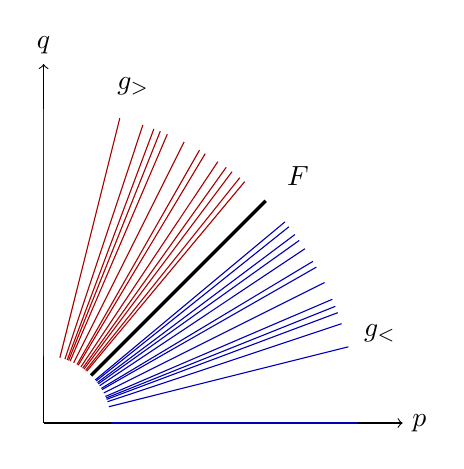
\begin{tikzpicture}[scale=0.95,
  low/.style={blue!70!black,thin},high/.style={red!65!black,thin},diag/.style={black,very thick}]
\draw[->] (0,0) -- (4.8,0) node[right] {$p$};
\draw[->] (0,0) -- (0,4.8) node[above] {$q$};
\draw[high] (0.000,0.900) -- (0.000,4.200);
\draw[low] (0.900,0.000) -- (4.200,0.000);
\draw[diag] (0.636,0.636) -- (2.970,2.970);
\draw[high] (0.402,0.805) -- (1.878,3.757);
\draw[high] (0.285,0.854) -- (1.328,3.984);
\draw[high] (0.218,0.873) -- (1.019,4.075);
\draw[low] (0.805,0.402) -- (3.757,1.878);
\draw[high] (0.499,0.749) -- (2.330,3.495);
\draw[high] (0.334,0.836) -- (1.560,3.900);
\draw[low] (0.854,0.285) -- (3.984,1.328);
\draw[low] (0.749,0.499) -- (3.495,2.330);
\draw[high] (0.540,0.720) -- (2.520,3.360);
\draw[high] (0.463,0.772) -- (2.161,3.601);
\draw[high] (0.355,0.827) -- (1.654,3.860);
\draw[high] (0.316,0.843) -- (1.475,3.933);
\draw[low] (0.873,0.218) -- (4.075,1.019);
\draw[low] (0.720,0.540) -- (3.360,2.520);
\draw[high] (0.562,0.703) -- (2.624,3.280);
\draw[high] (0.447,0.781) -- (2.084,3.647);
\draw[low] (0.836,0.334) -- (3.900,1.560);
\draw[low] (0.772,0.463) -- (3.601,2.161);
\draw[low] (0.703,0.562) -- (3.280,2.624);
\draw[high] (0.576,0.691) -- (2.689,3.227);
\draw[high] (0.523,0.732) -- (2.441,3.418);
\draw[low] (0.691,0.576) -- (3.227,2.689);
\draw[low] (0.827,0.355) -- (3.860,1.654);
\draw[low] (0.781,0.447) -- (3.647,2.084);
\draw[low] (0.732,0.523) -- (3.418,2.441);
\draw[low] (0.843,0.316) -- (3.933,1.475);
\node at (3.4,3.3) {$F$};
\node at (4.5,1.2) {$\gl$};
\node at (1.2,4.5) {$\gr$};
\end{tikzpicture}
\caption{The rays $r=(p,q)$ whose function in the ascending factorization
of $T^5$ has a nonzero coefficient in total degree at most $12$ (that is,
$[t^j]\varphi_r\neq0$ for some $j\geq1$ with $j|r|\leq12$), computed by
the construction in the proof of Proposition~\ref{prop:KS}. Blue: slope
below $1$, the factors of $\gl$ ($h<0$). Red: slope above $1$, the
factors of $\gr$ ($h>0$). Thick black: the diagonal, whose function is
$F$. Each ray is drawn from radius $0.9$ to $4.2$ for legibility.
The proof uses only the sign of $h$ on each side of the diagonal.}
\label{fig:rays}
\end{figure}

\section{The \texorpdfstring{$h$}{h}-grading and the extraction of the diagonal}\label{sec:filtration}

This section introduces the grading that separates the two sides of the
diagonal and shows that $\gl^{-1}(s)$ has only three graded components.
Throughout, $A=\ps{u,w}$ and $t=uw$; we identify $\ps{t}$ with the
subring of $A$ of series in $uw$.

For a monomial put $h(u^pw^q)=q-p$, and for $k\in\mathbb{Z}$ let $\pi_k$
be the continuous projection of $A$ onto the closed span of the monomials
with $h=k$. The monomials with $h=0$ are the powers of $t$, so
$\pi_0(A)=\ps{t}$, and $\pi_{-1}(A)=u\ps{t}$, $\pi_1(A)=w\ps{t}$. Let
$\Oge{k}$ and $\Ole{k}$ be the closed subspaces of series all of whose
monomials have $h\geq k$, respectively $h\leq k$. Since $h$ is additive,
$\Oge0$ is a closed subring, $\Oge{k}\Oge{l}\subseteq\Oge{k+l}$, and
likewise for $\Ole{}$; in particular $1+\Oge1$ and $1+\Ole{-1}$ are
groups under multiplication.

Group the factorization of $T^5$ by slope: let $\gl$ be the ascending
product of the walls $\theta_{r,\varphi_r}$ with $r_2<r_1$ (including
$(1,0)$), let $\gr$ be that of the walls with $r_2>r_1$ (including
$(0,1)$), and let $\theta_F=\theta_{(1,1),F}$, so that
\begin{equation}\label{eq:split}
  T^5=\gl\circ\theta_F\circ\gr,\qquad
  \theta_F(u)=uF(t),\quad \theta_F(w)=w/F(t).
\end{equation}
The automorphisms $\gl$ and $\gr$ are Poisson, by Lemma~\ref{lem:walls}.
The following theorem, the core of the proof, is proved in
Sections~\ref{sec:filtration}--\ref{sec:solution}.

\begin{theorem}\label{thm:mainlemma}
Let $F\in\Lambda$, let $\theta_F$ be as in \eqref{eq:split}, and let
$\gl,\gr$ be Poisson automorphisms of $A=\ps{u,w}$ such that, for every
$a\in\N^2$,
\begin{equation}\label{eq:filt}
  \gr(z^a)\in z^a(1+\Oge1),\qquad \gl^{-1}(z^a)\in z^a(1+\Ole{-1}),
\end{equation}
and such that $T^5=\gl\circ\theta_F\circ\gr$. Then $F=\Sst^{5}$, where
$\Sst=(1+\xi)/(1-\xi-\xi^2)$ and $\xi\in t\ps{t}$ is the unique series
with $\xi=t+\xi^2+\xi^3$.
\end{theorem}

\begin{lemma}\label{lem:filt}
The factors in \eqref{eq:split} satisfy \eqref{eq:filt}, and $\theta_F$
commutes with every projection $\pi_k$.
\end{lemma}

\begin{proof}
Let $\mathcal{G}_>$ be the set of unipotent automorphisms $g$ with
$g(z^a)\in z^a(1+\Oge1)$ for all $a$. A wall with $r_2>r_1$ lies in
$\mathcal{G}_>$, because $f(z^r)^{\omega(a,r)}-1$ is a series in the
monomials $z^{jr}$, $j\geq1$, which have $h=j(r_2-r_1)\geq1$. If
$g,g'\in\mathcal{G}_>$ and $g(z^a)=z^a(1+\eta)$ with $\eta\in\Oge1$, then
$g'g(z^a)=g'(z^a)\,(1+g'(\eta))$, and $g'(\eta)\in\Oge1$ because $g'$ maps each
monomial $z^k$ with $h(k)\geq1$ into $z^k(1+\Oge1)\subseteq\Oge1$ and is
continuous. So $\mathcal{G}_>$ is closed under composition, and it is
closed under $\m$-adic limits because its defining condition concerns
coefficients only. Hence $\gr\in\mathcal{G}_>$. The same argument, with
the inverse walls $\theta_{r,1/f}$, $r_2<r_1$, taken in descending order,
gives the statement for $\gl^{-1}$. Finally,
$\theta_F(z^a)=z^aF(t)^{a_1-a_2}$ has the same $h$ as $z^a$ in every
term.
\end{proof}

\begin{lemma}\label{lem:extract}
Under the hypotheses of Theorem~\ref{thm:mainlemma}, the series
$P=\gl^{-1}(s)$, $s=u+w$, has the form
\[
  P=uF(t)+\beta(t)+w\qquad\text{for some }\beta\in t\ps{t}.
\]
\end{lemma}

\begin{proof}
By Lemma~\ref{lem:Texplicit}, $T^5(s)=s$, so
$P=\gl^{-1}T^5(s)=\theta_F\gr(s)$. Write $\gr(u)=u(1+b_1)$ and
$\gr(w)=w(1+b_2)$ with $b_i\in\Oge1$. Then
\[
  P=\theta_F\gr(s)=uF\,\theta_F(1+b_1)+wF^{-1}\theta_F(1+b_2),
\]
where $uF\theta_F(b_1)\in\Oge0$ and the last term lies in $\Oge1$, by
Lemma~\ref{lem:filt}. So $\pi_{-1}(P)=uF$ and $\pi_k(P)=0$ for $k\leq-2$.
On the other side, $\gl^{-1}(u)=u(1+\eta_1)$ and $\gl^{-1}(w)=w(1+\eta_2)$ with
$\eta_i\in\Ole{-1}$, so $P=u(1+\eta_1)+w(1+\eta_2)$ has $\pi_1(P)=w$ and
$\pi_k(P)=0$ for $k\geq2$. Hence $P=uF+\pi_0(P)+w$, and
$\beta=\pi_0(P)\in\ps{t}$ has no constant term because $P\in\m$.
\end{proof}

\section{Splitting the logarithm}\label{sec:split}

This section turns the factorization into two identities, one for $F$
and one for $\gl$, by comparing graded components. For a unipotent
automorphism $\phi$ of $A$ let
\[
  \mu_\phi=\frac{\phi(u)/u}{\phi(w)/w}\in1+\m .
\]
Since $\phi\psi(u)/u=\phi\big(\psi(u)/u\big)\cdot\phi(u)/u$, and
likewise for $w$, these ratios satisfy the cocycle rule
$\mu_{\phi\psi}=\phi(\mu_\psi)\,\mu_\phi$.

\begin{lemma}\label{lem:cocycle}
Under the hypotheses of Theorem~\ref{thm:mainlemma},
\begin{equation}\label{eq:cocycle}
  (1+P)^5\,\mu_{\gl^{-1}}=F^2\,\theta_F(\mu_{\gr}),
\end{equation}
with $\mu_{\gl^{-1}}\in1+\Ole{-1}$ and $\theta_F(\mu_{\gr})\in1+\Oge1$.
\end{lemma}

\begin{proof}
By Lemma~\ref{lem:Texplicit}, $\mu_T=1+s$, and since $T$ fixes $s$, the
cocycle rule gives $\mu_{T^5}=(1+s)^5$. Also $\mu_{\theta_F}=F^2$. Apply
the cocycle rule to both sides of $\gl^{-1}T^5=\theta_F\gr$: the left side
gives $\gl^{-1}((1+s)^5)\,\mu_{\gl^{-1}}=(1+P)^5\mu_{\gl^{-1}}$, and the
right side gives $\theta_F(\mu_{\gr})\,F^2$. The two memberships follow
from \eqref{eq:filt}, applied to $u$ and $w$, and Lemma~\ref{lem:filt}.
\end{proof}

\begin{lemma}\label{lem:quadratic}
Let $F\in\Lambda$ and $\beta\in t\ps{t}$. There are
$\rho,\delta\in\Lambda$ with $\rho\delta=F$ and $\rho+t\delta=1+\beta$.
For such $\rho,\delta$,
\begin{equation}\label{eq:factor1P}
  1+uF(t)+\beta(t)+w=(1+u\delta)\cdot\rho\cdot(1+w/\rho)\qquad\text{in }A.
\end{equation}
\end{lemma}

\begin{proof}
The equation $\rho^2-(1+\beta)\rho+tF=0$ has a root $\rho\in\Lambda$: its
coefficient of $t^k$ is $\rho_k$ plus a polynomial in
$\rho_1,\dots,\rho_{k-1}$, so the coefficients are determined
recursively. Put $\delta=F/\rho$; then $\rho+t\delta=(\rho^2+tF)/\rho=1+\beta$.
Finally $(1+u\delta)(\rho+w)=\rho+w+u\rho\delta+uw\delta=1+\beta+uF+w$.
\end{proof}

\begin{proposition}\label{prop:E}
Under the hypotheses of Theorem~\ref{thm:mainlemma}, let $\beta$ be as in
Lemma~\ref{lem:extract} and $\rho,\delta$ as in Lemma~\ref{lem:quadratic}.
Then
\[
  F^2=\rho^5,\qquad \delta^2=\rho^3,\qquad \mu_{\gl^{-1}}=(1+u\delta)^{-5}.
\]
\end{proposition}

\begin{proof}
The logarithm is a continuous isomorphism from the multiplicative group
$1+\m$ onto the additive group $\m$, and it maps $1+\Ole{-1}$ into
$\Ole{-1}$ and $1+\Oge1$ into $\Oge1$, since these are closed and
stable under products. Take logarithms in \eqref{eq:cocycle}, using
Lemma~\ref{lem:extract} and \eqref{eq:factor1P}:
\[
  5\log(1+u\delta)+5\log\rho+5\log(1+w/\rho)+\log\mu_{\gl^{-1}}
  =2\log F+\log\theta_F(\mu_{\gr}).
\]
Here $u\delta\in\Ole{-1}$ and $w/\rho\in\Oge1$, so the terms lie in
$\Ole{-1}$, $\ps{t}$, $\Oge1$, $\Ole{-1}$, $\ps{t}$ and $\Oge1$
respectively. Applying $\pi_0$ gives $5\log\rho=2\log F$, that is,
$F^2=\rho^5$; then $\rho^2\delta^2=F^2=\rho^5$ gives $\delta^2=\rho^3$.
Applying $\sum_{k<0}\pi_k$ gives $5\log(1+u\delta)+\log\mu_{\gl^{-1}}=0$.
\end{proof}

\section{The string equation and a differential equation}\label{sec:string}

This section uses the Poisson property of $\gl$ to obtain a differential
equation for $(\rho,\delta)$, and shows that the equation has only one
solution. Let $E=u\partial_u+w\partial_w$ be the Euler derivation of $A$.
For $G\in\ps{t}$ write $G'=t\,dG/dt$. One checks directly that
\begin{equation}\label{eq:rules}
  E(G)=2G',\qquad \{G,u\}=-uG',\qquad \{G,w\}=wG',\qquad \{u,w\}=uw .
\end{equation}

\begin{lemma}\label{lem:euler}
Let $\phi$ be a unipotent Poisson automorphism of $A$. Then for all
$y\in A$,
\[
  \phi(E(y))=E(\phi(y))+\{\log\mu_\phi,\phi(y)\}.
\]
\end{lemma}

\begin{proof}
From the definition of the bracket, $uw\,E(y)=w\{u,y\}-u\{w,y\}$. Apply
$\phi$ and write $\phi(u)=u\alpha$, $\phi(w)=w\alpha'$. Expanding
$\{u\alpha,\phi y\}$ and $\{w\alpha',\phi y\}$ by the Leibniz rule and
using the same identity for $\phi(y)$ gives
$uw\alpha\alpha'\,\phi(E y)=uw\alpha\alpha'\big(E(\phi y)+\{\alpha,\phi y\}/\alpha-\{\alpha',\phi y\}/\alpha'\big)$.
Divide by $uw\alpha\alpha'$, and note that
$\{\alpha,g\}/\alpha-\{\alpha',g\}/\alpha'=\{\log(\alpha/\alpha'),g\}$.
\end{proof}

Formally, $E$ is the Hamiltonian derivation of $\log u-\log w$, and
Lemma~\ref{lem:euler} says that $\phi$ shifts $\log(u/w)$ by
$\log\mu_\phi$; the lemma makes this precise without logarithms of $u$
and $w$.

\begin{proposition}[String equation]\label{prop:string}
Under the hypotheses of Theorem~\ref{thm:mainlemma}, with $P$ as in
Lemma~\ref{lem:extract} and $\delta$ as in Lemma~\ref{lem:quadratic},
\[
  (1+u\delta)\big(E(P)-P\big)=5\,\{u\delta,P\}.
\]
\end{proposition}

\begin{proof}
The inverse of a Poisson automorphism is Poisson. Apply
Lemma~\ref{lem:euler} with $\phi=\gl^{-1}$ and $y=s$. Since $E(s)=s$ and
$\phi(s)=P$, and $\log\mu_\phi=-5\log(1+u\delta)$ by
Proposition~\ref{prop:E}, it gives
$P=E(P)-5\{u\delta,P\}/(1+u\delta)$.
\end{proof}

\begin{lemma}\label{lem:exact}
For $\rho,\delta\in\ps{t}$ put $P=(\rho+w)(1+u\delta)-1$, and
\[
  \Phi(\rho,\delta)=1-\rho+2\rho'-4t\delta-3t\delta',\qquad
  \Psi(\rho,\delta)=2\rho\delta'-3\delta\rho' .
\]
Then $(1+u\delta)(E(P)-P)-5\{u\delta,P\}=(1+u\delta)\big(\Phi(\rho,\delta)+u\,\Psi(\rho,\delta)\big)$.
\end{lemma}

\begin{proof}
Expand the left side with the Leibniz rule and \eqref{eq:rules}; a
direct computation shows that it equals the right side.
\end{proof}

\begin{corollary}\label{cor:ode}
Under the hypotheses of Theorem~\ref{thm:mainlemma}, the series $\rho$ and
$\delta$ of Proposition~\ref{prop:E} satisfy $\delta^2=\rho^3$ and
\begin{equation}\label{eq:ode}
  1-\rho+2\rho'-4t\delta-3t\delta'=0 .
\end{equation}
\end{corollary}

\begin{proof}
By Lemma~\ref{lem:extract} and \eqref{eq:factor1P},
$P=(\rho+w)(1+u\delta)-1$. Proposition~\ref{prop:string} and
Lemma~\ref{lem:exact} give $(1+u\delta)(\Phi+u\Psi)=0$. As $1+u\delta$ is
a unit, $\Phi+u\Psi=0$; the term $\Phi$ has $h=0$ and $u\Psi$ has $h=-1$,
so $\Phi=0$.
\end{proof}

Since $\delta=\rho^{3/2}$, equation \eqref{eq:ode} is the first-order
equation $2\rho'-\rho+1-3(t\rho^{3/2})'-t\rho^{3/2}=0$ for $\rho$ alone.

\begin{lemma}\label{lem:unique}
There is at most one pair $(\rho,\delta)\in\Lambda^2$ with $\delta^2=\rho^3$
satisfying \eqref{eq:ode}.
\end{lemma}

\begin{proof}
Write $\rho=\sum\rho_kt^k$ and $\delta=\sum\delta_kt^k$, with
$\rho_0=\delta_0=1$. For $k\geq1$ the coefficient of $t^k$ in
\eqref{eq:ode} is $(2k-1)\rho_k-(3k+1)\delta_{k-1}$. The coefficient of
$t^n$ in $\delta^2=\rho^3$ reads $2\delta_n=3\rho_n+{}$(a polynomial in
$\rho_1,\dots,\rho_{n-1},\delta_1,\dots,\delta_{n-1}$). By induction,
$\delta_{k-1}$ is determined by $\rho_1,\dots,\rho_{k-1}$, and then
$\rho_k=(3k+1)\delta_{k-1}/(2k-1)$, since $2k-1\neq0$.
\end{proof}

\section{The solution and the proof of the theorem}\label{sec:solution}

This section exhibits the solution of \eqref{eq:ode}, completes the proofs
of Theorems~\ref{thm:mainlemma} and~\ref{thm:main}, and derives the
binomial sum.

Let $\xi\in t\ps{t}$ be the unique series with $\xi(1-\xi-\xi^2)=t$,
equivalently $\xi=t+\xi^2+\xi^3$, and let
\[
  \Sst=\frac{1+\xi}{1-\xi-\xi^2}=\frac1t-\frac1\xi .
\]
(The second expression holds because $1/\xi=(1-\xi-\xi^2)/t$.) Since
$\xi=t+O(t^2)$, the substitution $t\mapsto\xi$ identifies $\ps{t}$ with
$\ps{\xi}$.

\begin{lemma}\label{lem:solution}
The pair $(\rho,\delta)=(\Sst^2,\Sst^3)$ lies in $\Lambda^2$, satisfies
$\delta^2=\rho^3$ and solves \eqref{eq:ode}. Moreover $\Sst$ satisfies
\eqref{eq:cubic}, and it is the only series in $\Lambda$ that does.
\end{lemma}

\begin{proof}
As $dt/d\xi=(1+\xi)(1-3\xi)$ is a unit, $G'=t\,(dG/d\xi)/(dt/d\xi)$ for
$G\in\ps{t}$, and
\[
  \Sst'=\frac{\xi(2+2\xi+\xi^2)}{(1+\xi)(1-3\xi)(1-\xi-\xi^2)} .
\]
With $(\Sst^2)'=2\Sst\Sst'$ and $(\Sst^3)'=3\Sst^2\Sst'$, the left side of
\eqref{eq:ode} becomes $1-\Sst^2+4\Sst\Sst'-4t\Sst^3-9t\Sst^2\Sst'$, a
rational function of $\xi$ whose denominator is a product of the units
$1+\xi$, $1-3\xi$, $1-\xi-\xi^2$; a direct computation shows that it is
$0$. Substituting $t=\xi(1-\xi-\xi^2)$ and $\Sst$ into \eqref{eq:cubic}
likewise gives $0$. For uniqueness, the coefficient of $t^k$ in
\eqref{eq:cubic} is $S_k$ plus a polynomial in $S_0,\dots,S_{k-1}$.
\end{proof}

\begin{proof}[Proof of Theorem~\ref{thm:mainlemma}]
By Corollary~\ref{cor:ode}, Lemma~\ref{lem:solution} and
Lemma~\ref{lem:unique}, $\rho=\Sst^2$ and $\delta=\Sst^3$. Hence
$F=\rho\delta=\Sst^5$.
\end{proof}

\begin{lemma}\label{lem:lagrange}
For $j\geq1$,
\[
  [t^j]\,\Sst=\frac1j\,[z^{j+1}]\,(1-z-z^2)^{-j}
  =\frac1j\sum_{\ell}\binom{j+\ell-1}{\ell}\binom{\ell}{j+1-\ell}.
\]
\end{lemma}

\begin{proof}
The series $\xi$ satisfies $\xi=t\,R(\xi)$ with $R(z)=(1-z-z^2)^{-1}$.
Lagrange inversion for integer powers \cite[Theorem~2.1.1 and
(2.2.1)]{Gessel} gives $[t^n]\,\xi^k=\frac kn[z^{n-k}]R(z)^n$ for all
integers $k$ and $n\neq0$. With $k=-1$ and $n=j$, and since
$\Sst=1/t-1/\xi$, this gives the first equality. For the second, expand
$(1-z(1+z))^{-j}=\sum_{\ell\geq0}\binom{j+\ell-1}{\ell}z^\ell(1+z)^\ell$
and take the coefficient of $z^{j+1}$.
\end{proof}

\begin{proof}[Proof of Theorem~\ref{thm:main}]
By Lemma~\ref{lem:filt}, the factorization \eqref{eq:split} of $T^5$
satisfies the hypotheses of Theorem~\ref{thm:mainlemma}, so $F=\Sst^5$.
By \eqref{eq:SF}, $S^5=\Sst^5$. Fifth roots in $\Lambda$ are unique (if
$G_1,G_2\in\Lambda$ and $G_1^5=G_2^5$, then $G_1/G_2\in\Lambda$ is a fifth root of
unity with constant term $1$, hence $G_1/G_2=1$), so $S=\Sst$.
Lemma~\ref{lem:lagrange} gives \eqref{eq:ers}; the term with index $\ell$
vanishes unless $0\leq j+1-\ell\leq\ell$, that is,
$\lceil(j+1)/2\rceil\leq\ell\leq j+1$. Lemma~\ref{lem:solution} gives
\eqref{eq:cubic} and its uniqueness.
\end{proof}

\begin{remark}[Algebraicity]\label{rem:algebraic}
In particular, the wall function $S(x^2y^5)$ on the ray $(2,5)$ of
$\mathfrak{D}(1+x,1+y^5)$ is algebraic over $\Q(x^2y^5)$, by
\eqref{eq:cubic}. Burcroff, Lee, Mou, Musiker and Reineke deduced this,
and an exponential growth rate $27/5$ of the coefficients, from the
conjectured formula \cite[\S9.3]{BLMMR}, in connection with the question,
which they attribute to Kontsevich, whether every wall function of a
cluster scattering diagram is algebraic. Theorem~\ref{thm:main} makes
both statements unconditional for this ray.
\end{remark}

\begin{remark}[Other exponents]\label{rem:general}
Sections~\ref{sec:T}--\ref{sec:string} do not use the value $5$ except
through the exponent of $T$. For an integer $c\geq1$ the same argument
applies to $T^c$ and the ray $(2,1)$ of $\mathfrak{D}((1+t)^c,1+t)$: it
shows that this ray carries $\rho_c^{c/2}$, where $\rho_c\in\Lambda$ is
the unique solution of
\[
  2\rho'-\rho+1-(c-2)\big(t\rho^{c/2-1}\big)'-t\rho^{c/2-1}=0 .
\]
This general form is a by-product of the written argument and is not
part of the formalization, which treats $c=5$ only; for $c=3,6,7$ it
agrees with the factorization of $T^c$ through order $t^5$.
\end{remark}

\section{Formalization}\label{sec:lean}

This section states what is checked in Lean and what is trusted. The
Lean development accompanying this paper (folder \texttt{lean/}) is
written in Lean~4 (version 4.32.2) with Mathlib, and builds in a few
minutes with the Mathlib cache.

\subsection*{The statement}
The main theorem is \texttt{ErsConj13.ers\_conjecture\_13} in
\texttt{lean/Main.lean}:
{\small
\begin{verbatim}
theorem ers_conjecture_13 :
    (∃ f, IsConsistentFamily (1 + PowerSeries.X) (1 + PowerSeries.X ^ 5) f) ∧
    ∀ f, IsConsistentFamily (1 + PowerSeries.X) (1 + PowerSeries.X ^ 5) f →
      ∀ j, 1 ≤ j → PowerSeries.coeff j (f ((5 / 2 : ℚ≥0) : Slope)) = ersCoeff j
\end{verbatim}
}
\noindent It states that $\mathfrak{D}(1+t,1+t^5)$ has a consistent family,
so that the second part is not vacuous, and that for every consistent
family $f$ and every $j\geq1$ the coefficient of $t^j$ in the function on
the ray of slope $5/2$, the ray $(2,5)$, equals the right side of
\eqref{eq:ers}. The definitions it uses are in
\texttt{lean/ErsConj13/ScatDefs.lean} and
\texttt{lean/ErsConj13/Defs.lean}:
\begin{itemize}
\item \texttt{Slope} is $\mathbb{Q}_{\geq0}$ with a top element added; a slope
$q/p$ in lowest terms stands for the ray $(p,q)$, and the top element
for $(0,1)$. A family is a function from slopes to $\ps{t}$.
\item \texttt{wall s f} is the substitution \eqref{eq:wall} on $\ps{x,y}$.
\item \texttt{IsConsistentFamily P$_1$ P$_2$ f} holds when every
$f_r$ has constant term $1$ and, for every $N$ and each of $x,y$, the
finite ascending product of the walls with $r_1+r_2<N$ agrees with
$\theta_{(0,1),P_2}\theta_{(1,0),P_1}$ on that generator in all
coefficients of total degree less than $N$. This is
Definition~\ref{def:consistent}, with the infinite product read degree by
degree as in Section~\ref{sec:defs}.
\item \texttt{ersCoeff j} is
$\frac1j\sum_{\ell=0}^{j+1}\binom{\ell}{j+1-\ell}\binom{j+\ell-1}{\ell}$,
the right side of \eqref{eq:ers} (the subtractions are of natural numbers
and do not truncate for $j\geq1$, $\ell\leq j+1$), and \texttt{S} is
$1+\sum_{j\geq1}\texttt{ersCoeff j}\,t^j$.
\end{itemize}

\subsection*{What is proved}
The Lean development assumes nothing beyond the definitions: the ordered
factorization, the change of lattice and the uniqueness of the solution of \eqref{eq:ode} are
all proved. The main intermediate results are
\texttt{ErsConj13.ray21\_eq\_S5} in \texttt{lean/Realization.lean}
($\mathfrak{D}_5$ has a consistent family, and its function on the ray
$(2,1)$ is $\texttt{S}^5$) and \texttt{ErsConj13.main\_lemma} in
\texttt{lean/MainLemma.lean} (Theorem~\ref{thm:mainlemma}, with the
conclusion $F=\texttt{S}^5$). The table lists the Lean names of the other
steps; supporting lemmas are in \texttt{lean/ErsConj13/}. Small checks of
the definitions, such as the first values of \texttt{ersCoeff}, are in
\texttt{lean/Examples.lean}.

\begin{center}
\small
\begin{tabular}{ll}
\toprule
In this paper & In the Lean development\\
\midrule
Lemma~\ref{lem:walls} & \texttt{wall\_bracket}\\
Proposition~\ref{prop:KS} & \texttt{factor\_exists}, \texttt{factor\_unique}\\
Proposition~\ref{prop:lattice} & \texttt{transport5\_consistent}\\
Proposition~\ref{prop:T5} & \texttt{transport\_consistent}\\
Lemma~\ref{lem:filt} & \texttt{realization}\\
Lemma~\ref{lem:extract} & \texttt{V1}\\
Lemmas~\ref{lem:cocycle}, \ref{lem:quadratic}, Proposition~\ref{prop:E} & \texttt{cocycle}, \texttt{quad\_root}, \texttt{one\_add\_P\_factor}, \texttt{lemma\_E}\\
Lemma~\ref{lem:euler}, Proposition~\ref{prop:string} & \texttt{euler\_conj}, \texttt{lemma\_SE}\\
Lemma~\ref{lem:exact}, Corollary~\ref{cor:ode} & \texttt{exact\_identity}, \texttt{ode\_of\_SE}\\
Lemma~\ref{lem:unique} & \texttt{ode\_unique}\\
Lemma~\ref{lem:solution} & \texttt{c5\_identity}, \texttt{S\_cubic}\\
\bottomrule
\end{tabular}
\end{center}

The formal proof differs from the text in two places. It avoids
logarithms: the comparison of graded components in
Proposition~\ref{prop:E} is replaced by the uniqueness of factorizations
in $(1+\Ole{-1})\cdot\ps{t}^{\times}\cdot(1+\Oge1)$ applied to
\eqref{eq:cocycle} directly (\texttt{unique\_factor}), and
Lemma~\ref{lem:euler} is used in a form multiplied through by
$\phi(u)\phi(w)/(uw)$. And it works with $\texttt{S}$, defined by the
binomial sum, rather than with $\Sst$: it proves that $\texttt{S}$
satisfies \eqref{eq:cubic} by showing that its coefficients and those of
the root of \eqref{eq:cubic} satisfy the same second-order linear
recurrence with the same initial values (for the sequence A217596 this
recurrence was recorded by Peter Bala in 2015 \cite{OEIS}), and then derives \eqref{eq:ode} for
$(\texttt{S}^2,\texttt{S}^3)$ from \eqref{eq:cubic}. Lagrange inversion
is therefore not used in the formal proof.

\subsection*{Axioms and trust}
During the build, the file \texttt{lean/Axioms.lean} checks that
\texttt{ers\_conjecture\_13} and the main intermediate theorems use no
axioms beyond the three standard ones of Lean and Mathlib:
\texttt{propext}, \texttt{Classical.choice} and \texttt{Quot.sound}. The trusted base is Lean's kernel, Mathlib, and
the faithfulness of the definitions above to the coefficients
$\tau^{1,5}$ of \cite[(2.2)]{BLMMR}: Definition~\ref{def:consistent} is the
consistency condition of \cite[\S1.3]{GPS} by Remark~\ref{rem:GPS}, the
levelwise reading of the infinite product is equivalent to the
$\m$-adic one, and the ray of slope $5/2$ is the ray $(2,5)$ of
Definition~\ref{def:tau}. The identification of these coefficients with
those of \cite{ERS} is the reading explained in
Remark~\ref{rem:reading}. As a check of conventions, separate from the
proof, the values $\tau^{1,5}(2j,j)$ for $j\leq12$ produced by the code
published with \cite{ERS} (see \cite{scatcoef}) agree with \eqref{eq:ers}.

\begin{thebibliography}{99}

\bibitem{Akagi}
R.~Akagi,
\emph{Some coefficients of rank 2 cluster scattering diagrams},
preprint, 2025.
\href{https://arxiv.org/abs/2507.21916}{arXiv:2507.21916}.

\bibitem{Akagi23}
R.~Akagi,
\emph{Explicit forms in lower degrees of rank 2 cluster scattering diagrams},
Algebr. Comb. \textbf{8} (2025), no.~4, 1021--1067.
\href{https://doi.org/10.5802/alco.432}{doi:10.5802/alco.432};
\href{https://arxiv.org/abs/2309.15470}{arXiv:2309.15470}.

\bibitem{BL}
A.~Burcroff and K.~Lee,
\emph{Broken lines and compatible pairs for rank 2 quantum cluster algebras},
Selecta Math. (N.S.) \textbf{32} (2026), no.~4, Paper No.~81.
\href{https://doi.org/10.1007/s00029-026-01189-z}{doi:10.1007/s00029-026-01189-z};
\href{https://arxiv.org/abs/2404.14369}{arXiv:2404.14369}.

\bibitem{BLM}
A.~Burcroff, K.~Lee and L.~Mou,
\emph{Scattering diagrams, tight gradings, and generalized positivity},
Proc. Natl. Acad. Sci. USA \textbf{122} (2025), no.~18, e2422893122.

\bibitem{BLMMR}
A.~Burcroff, K.~Lee, L.~Mou, G.~Musiker and M.~Reineke,
\emph{Cluster scattering diagrams via quiver moduli and tight gradings},
J. Lond. Math. Soc. (2) \textbf{114} (2026), no.~2, e70642.
\href{https://doi.org/10.1112/jlms.70642}{doi:10.1112/jlms.70642};
\href{https://arxiv.org/abs/2511.14672}{arXiv:2511.14672}.
Section and equation numbers refer to arXiv version~1.

\bibitem{ERS}
T.~Elgin, N.~Reading and S.~Stella,
\emph{Cluster scattering coefficients in rank 2},
Arnold Math. J. \textbf{12} (2026), no.~1, 111--122.
\href{https://doi.org/10.56994/armj.012.001.003}{doi:10.56994/armj.012.001.003};
\href{https://arxiv.org/abs/2404.11381}{arXiv:2404.11381}.
Section numbers refer to arXiv version~4.

\bibitem{scatcoef}
T.~Elgin, N.~Reading and S.~Stella,
\emph{scatcoef}, computer code accompanying \cite{ERS},
\url{https://github.com/Etn40ff/scatcoef}.

\bibitem{Gessel}
I.~M.~Gessel,
\emph{Lagrange inversion},
J. Combin. Theory Ser. A \textbf{144} (2016), 212--249.
\href{https://doi.org/10.1016/j.jcta.2016.06.018}{doi:10.1016/j.jcta.2016.06.018};
\href{https://arxiv.org/abs/1609.05988}{arXiv:1609.05988}.

\bibitem{GHKK}
M.~Gross, P.~Hacking, S.~Keel and M.~Kontsevich,
\emph{Canonical bases for cluster algebras},
J. Amer. Math. Soc. \textbf{31} (2018), no.~2, 497--608.
\href{https://doi.org/10.1090/jams/890}{doi:10.1090/jams/890};
\href{https://arxiv.org/abs/1411.1394}{arXiv:1411.1394}.

\bibitem{GPS}
M.~Gross, R.~Pandharipande and B.~Siebert,
\emph{The tropical vertex},
Duke Math. J. \textbf{153} (2010), no.~2, 297--362.
\href{https://doi.org/10.1215/00127094-2010-025}{doi:10.1215/00127094-2010-025};
\href{https://arxiv.org/abs/0902.0779}{arXiv:0902.0779}.

\bibitem{GS11}
M.~Gross and B.~Siebert,
\emph{From real affine geometry to complex geometry},
Ann. of Math. (2) \textbf{174} (2011), no.~3, 1301--1428.
\href{https://doi.org/10.4007/annals.2011.174.3.1}{doi:10.4007/annals.2011.174.3.1}.

\bibitem{KS06}
M.~Kontsevich and Y.~Soibelman,
\emph{Affine structures and non-Archimedean analytic spaces},
in: \emph{The Unity of Mathematics}, Progr. Math. \textbf{244},
Birkh\"auser, Boston, 2006, 321--385.
\href{https://doi.org/10.1007/0-8176-4467-9_9}{doi:10.1007/0-8176-4467-9\_9};
\href{https://arxiv.org/abs/math/0406564}{arXiv:math/0406564}.

\bibitem{KS08}
M.~Kontsevich and Y.~Soibelman,
\emph{Stability structures, motivic Donaldson--Thomas invariants and
cluster transformations}, preprint, 2008.
\href{https://arxiv.org/abs/0811.2435}{arXiv:0811.2435}.

\bibitem{OEIS}
V.~Kruchinin (with functional equations by P.~D.~Hanna, a recurrence by
P.~Bala, a comment and formulas by M.~S.~Saydam, and additions by others),
\emph{Expansion of g.f.\ $x/\mathrm{reversion}(x-x^2-x^3)$}, sequence
A217596 in The On-Line Encyclopedia of Integer Sequences, 2013,
\url{https://oeis.org/A217596}.

\bibitem{RW}
M.~Reineke and T.~Weist,
\emph{Refined GW/Kronecker correspondence},
Math. Ann. \textbf{355} (2013), no.~1, 17--56.
\href{https://doi.org/10.1007/s00208-012-0778-0}{doi:10.1007/s00208-012-0778-0};
\href{https://arxiv.org/abs/1103.5283}{arXiv:1103.5283}.

\end{thebibliography}
\end{document}
